\documentclass[a4paper,10pt,twoside]{article}
%\usepackage{amssymb}
%\usepackage{amsthm}
\usepackage[polish]{babel}
\usepackage[utf8]{inputenc}
\usepackage[T1]{fontenc}
\usepackage{indentfirst}
\usepackage[top=2.5cm, bottom=2.5cm, left=2.5cm, right=2.5cm]{geometry}
\usepackage{graphicx}
\usepackage{amsmath}
\usepackage[version=4]{mhchem}
\usepackage{adjustbox}

\begin{document}

\begin{center}
\bgroup
\def\arraystretch{1.5}
\begin{tabular}{|c|c|c|c|c|c|}
	\hline
	EAIiIB & \multicolumn{2}{|c|}{\begin{tabular}{@{}c@{}}Marcin Nalepa \\ Przemysław Trybała\end{tabular}} & Rok II & Grupa 5 & Zespół 3 \\
	\hline
	\multicolumn{3}{|c|}{\begin{tabular}{c}Temat: \\ Elektroliza \end{tabular}} & 
	\multicolumn{3}{|c|}{\begin{tabular}{c}Numer ćwiczenia: \\ 35 \end{tabular}} \\
	\hline
	\begin{tabular}{@{}c@{}}Data wykonania\\13.01.2016\end{tabular} & \begin{tabular}{@{}c@{}}Data oddania\\21.01.2016\end{tabular} & 
	\begin{tabular}{c}Zwrot do\\poprawki\\\phantom{data} \end{tabular} & \begin{tabular}{c}Data oddania\\\phantom{data}\end{tabular} &
	\begin{tabular}{@{}c@{}}Data zaliczenia\\\phantom{data}\end{tabular} & \begin{tabular}{c}Ocena\\\phantom{ocena}\end{tabular} \\[4ex]
	\hline
\end{tabular}
\egroup
\end{center}

\section{Cel ćwiczenia}
Celem ćwiczenia jest wyznaczenie stałej Faradaya, równoważnika elektrochemicznego miedzi oraz ładunku elementarnego metodą elektrolizy.

\section{Wstęp teoretyczny}
Elektrolity to charakterystyczna grupa przewodników. Elektrolit powstaje gdy struktura krystaliczna rozpuszczanej substancji, rozpada się (dysocjuje)
na jony, które następnie poruszają się bezładnie po roztworze. Gdy w elektrolicie zanurzymy elektrody i podłączymy je do źródła stałego prądu,
ruch jonów stanie się uporządkowany i zacznie płynąć przez niego prąd - kationy podążają do ujemnej katody, a aniony do anody.
Gdy jody dotrą do elektrody, zostają zobojętnione i odkładają się na niej jako grupy atomów. Proces ten jest zwany elektrolizą.

Aby jon mógł zostać zobojętniony na elektrodzie, musi przepłynąć ładunek równy $w*e$, gdzie $e$ - ładunek elementarny elektronu, a $w$ - wartościowość jonu.
Liczbę atomów które wydzieliły się na elektrodzie możemy wyznaczyć jako stosunek całkowitego ładunku ($I*t$) do ładunku pojedynczego jonu ($we$)
\begin{equation}
N=\frac{It}{we}
\end{equation}
Masę osadzonych atomów można obliczyć mnożąc ich ilość przez masę jednego atomu. Masę pojedynczego atomu można wyznaczyć jako stosunek masy molowej do
liczby Avogadra, stąd
\begin{equation}
\label{eq:masa}
m=N\frac{\mu}{N_A}=\frac{\mu}{weN_A}It
\end{equation}

Można zauważyć, że masa wydzielonej substancji jest proporcjonalna do natężenia prądu $I$, czasu przepływu prądu $t$ oraz współczynnika 
\begin{equation}
\label{eq:k}
k=\frac{\mu}{weN_A}
\end{equation}
oznaczanego $k$ i zwanego elektrochemicznym równoważnikiem substancji.

Iloczyn $eN_A$ wyraża ładunek potrzebny do wydzielenie jednego gramorównoważnika chemicznego substancji. Oznacza się go zwykle jako $F$ i nazywa stałą Faradaya.
Ze wzoru (\ref{eq:k}) wynika jego zależność od $k$:
\begin{equation}
%\label{eq:k}
F=\frac{\mu}{wk}
\end{equation}

\newpage
\section{Opis doświadczenia}
W doświadczeniu użyto roztworu siarczanu miedzi (II) \ce{CuSO4} jako elektrolitu oraz miedzianych elektrod, stąd warościowość $w=2$ ponieważ siarczan miedzi (II)
dysocjuje na \ce{CuSO4 ->[\ce{H2O}] Cu^2+ + SO4^2-}. Układ pomiarowy został przedstawiony na rysunku.
\begin{figure}[!htb]
\centerline{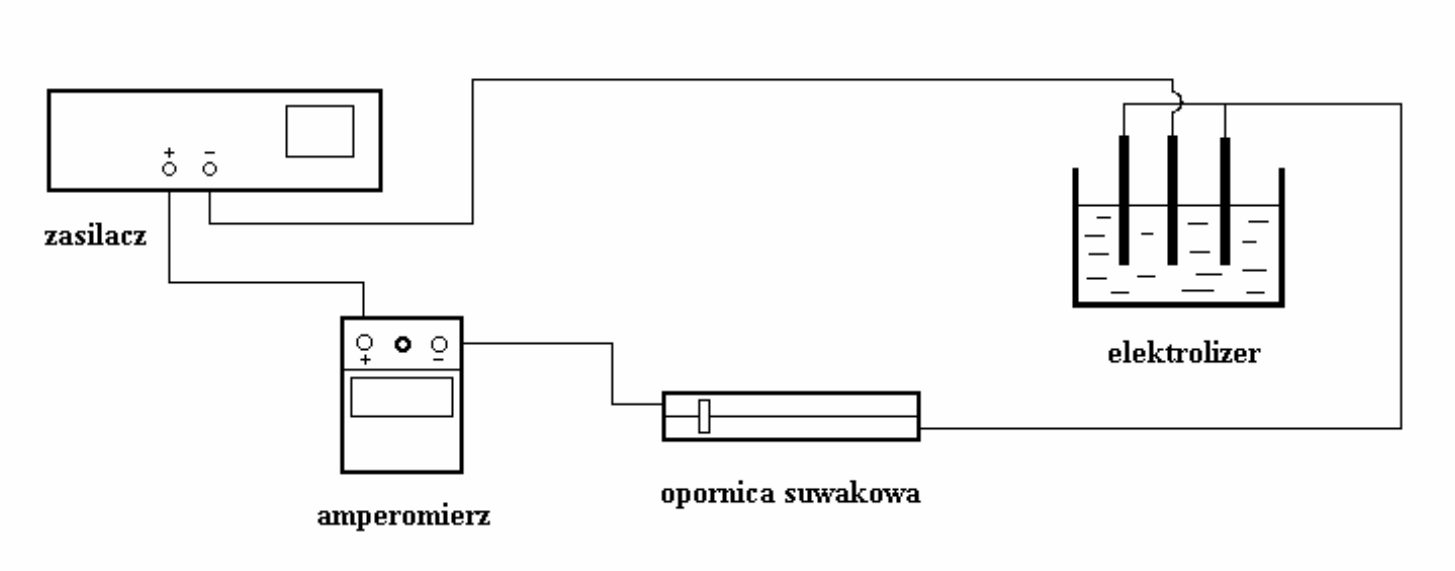
\includegraphics[scale=0.3]{scheme}}
\caption{Schemat wykorzystanego obwodu elektrycznego}
\end{figure}
Użyte elektrody zostały oczyszczone za pomocą papieru ściernego i wody destylowanej, osuszone, a następnie zważone. Po umocowaniu elektrod na statywie, zostały one
zanurzone w elektrolicie. Prąd płynący przez roztwór został ustalony na $0.6A$.

\section{Wyniki pomiarów}
\begin{table}[!htb]
\centering
\caption{Wyniki pomiarów}
\def\arraystretch{1.5}
\begin{tabular}{|r|r|r|r|}
\hline
\multicolumn{1}{|l|}{} & \multicolumn{1}{c|}{anoda 1} & \multicolumn{1}{c|}{anoda 2} & \multicolumn{1}{c|}{katoda} \\ \hline
masa przed $[g]$       & 100,544                      & 85,796                       & 134,391                     \\ \hline
$u(m)~[g]$             & 0,001                        & 0,001                        & 0,001                       \\ \hline
masa po $[g]$          & 100,346                      & 85,634                       & 134,764                     \\ \hline
$u(m)~[g]$             & 0,001                        & 0,001                        & 0,001                       \\ \hline
$\Delta m~[g]$         & 0,198                        & 0,160                        & 0,373                       \\ \hline
$u(\Delta m)~[g]$      & 0,01                         & 0,01                         & 0,01                        \\ \hline
\end{tabular}
\end{table}
\begin{itemize}
\item Czas trwania elektrolizy: $30~[min]=1800~[s]$
\item Natężenie prądu $I=0,6~A$
\end{itemize}
Niepewność $u(\Delta m)$ została przyjęta jako $0,01g$ ponieważ część miedzi mogła zostać spłukana z powierzchni elektrod
podczas przygotowywania ich do ważenia.

\newpage
\section{Opracowanie wyników}
\noindent
Obliczenie ubytku masy:
\begin{itemize}
\item Przyrost masy na katodzie: $134,764 - 134,391 = 0,373~[g]$
\item Ubytek masy na anodach: $100,544-100,346 + 85,796-85,636 = 0,360~[g]$
\item Wartość średnia $m= \frac{0,373+0,360}{2} \approx 0,367~[g]$
\end{itemize}
\vspace{5pt}
Obliczenia dla prądu:
\begin{itemize}
\item Natężenie prądu $I = 0,6A$
\item Niepewność: $u(I) = \frac{klasa * zakres}{100} = \frac{0,5*0,75}{100}=3,75~[mA]$
\end{itemize}

\noindent
stąd $I=600\pm 3,75~[mA]$

\vspace{10pt}
\noindent
Równoważnik liczymy ze wzoru
$$k=\frac{m}{It}=\frac{0,367}{0,6*1800}=0,3398~[mg]$$

\begin{align*}
	\frac{u(k)}{k} &= \sqrt{ \left(\frac{u(m)}{m} \right)^2 + \left(\frac{u(I)}{I} \right )^2 } \\
	&= \sqrt{ \left(\frac{0,01}{0,367} \right)^2 + \left(\frac{0,00375}{0,6} \right )^2 }=0,027
\end{align*}

$$u(k) = 0,027 * 0,3398~mg = 0,0092~mg$$

\noindent
Stałą Faradaya można obliczyć, przekształcając wzór (\ref{eq:k}):
\begin{align*}
	k&=\frac{\mu}{w*e*N_A} \\
	e*N_A&=\frac{\mu}{w*k},~~~F = e*N_A \\
	F&=\frac{\mu}{w*k}
\end{align*}
Dla jonów miedzi \ce{Cu^2+} $w$ wynosi 2, $\mu$ (masa molowa) wynosi $63,5\frac{g}{mol}$. Stąd mamy:
$$F=\frac{63,5}{2*0,3398*10^{-3}}=93600~[C]$$
W niepewności zmienną jest tylko k, więc wzór na niepewność dla stałej Faradaya liczonej ze wzoru $F=\frac{\mu}{n*k}$ wygląda następująco:
$$u(F)=F*\frac{u(k)}{k}=93600*0,027=2527~[C]$$
Ładunek elementarny możemy obliczyć przekształcając wzór $F=e*N_A$ do:
$$e=\frac{F}{N_A}$$
tak więc:
$$e=\frac{93600}{6,022*10^{-23}}=1,55*10^{-19}[C]$$
w niepewności liczonego ładunku elementarnego liczy się tylko obliczona stała Faradaya, tak więc liczymy ją ze wzoru:
$$u(e)=\sqrt{\left(\frac{\delta e}{\delta F}*u(F) \right)^2}=\frac{u(F)}{N_A}=\frac{2527}{6,022*10^{23}}=4,2*10^{-21}[C]$$


\newpage
\section{Podsumowanie}
%\begin{adjustbox}{center}
\begin{table}[!htb]
\centering
\def\arraystretch{1.5}
\begin{adjustbox}{center}
\begin{tabular}{|l|l|l|l|l|l|c|}
\hline
	& \begin{tabular}{@{}c@{}}Wartości\\obliczone\end{tabular}	& \begin{tabular}{@{}c@{}}Wartości\\tablicowe\end{tabular}
	& Różnica	& \begin{tabular}{@{}c@{}}Niepewność\\standardowa\end{tabular}
	& \begin{tabular}{@{}c@{}}Niepewność\\rozszerzona dla $k=2$\end{tabular} & \begin{tabular}{@{}c@{}}Zgodność z wartością\\tablicową $|x-x_0|<U(x)$\end{tabular}		\\ \hline
$k~[\frac{mg}{C}]$	& $0,3398$				& $0,329$					& $0,0108$  & $0,009$			& $0,018$			& tak						\\ \hline
$F~[C]$				& $93600$				& $96500$					& $2900$    & $2527$			& $5054$			& tak						\\ \hline
$e~[C]$				& $1,55*10^{-19}$		& $1,6021*10^{-19}$	& $5,2*10^{-21}$	& $4,2*10^{-21}$	& $8,4*10^{-21}$	& tak						\\ \hline
\end{tabular}
\end{adjustbox}
\end{table}

Obliczona wartość stałej Faradaya to $93600 \pm 2527~[C]$, a równoważnika elektrochemicznego miedzi $0,3398 \pm 0,009~[\frac{mg}{C}]$. Wartości te mieszczą się w niepewności rozszerzonej
i są zgodne z wartościami tablicowymi. Obliczona wartość ładunku elementarnego to $1,550*10^{-19} \pm 0,042*10^{-19}~[C]$, wartość ta również pokrywa się z wartościami tabelarycznymi.
Dzięki wysokiej dokładności pomiarów wszystkie obliczone wartości zgadzają się z oczekiwanymi.

\end{document}

























